\documentclass[12pt, oneside]{extbook} % the document type needs to be change
\usepackage{geometry}
\usepackage{listings}
\usepackage{graphicx}
\usepackage[dvipsnames]{xcolor}
\usepackage[utf8]{inputenc}
\usepackage[T1]{fontenc}
\usepackage[italian]{babel}


\lstset{
	language=C, 
	basicstyle=\ttfamily\small,
	keywordstyle=\color{purple}\bfseries\small,
	stringstyle=\color{ForestGreen}\small,
	commentstyle=\color{blue}\small,
	numbers=left,
	numberstyle=\small\color{black},
	numbersep=5pt,
	tabsize=2,
	showtabs=false,
	showspaces=false,
	showstringspaces=false,
	breaklines=true,
	keepspaces=true
}

\geometry{
    top = 1.5cm,
    bottom = 1.5cm,
    left = 2cm,
    right=2cm,
}

\begin{document}

\chapter*{Firewall and packet classification algorithm}

\section{Introduzione sul firewall}
Un firewall ispeziona un pacchetto in ingresso ed in base alle regole definite o le policies, decide se accettare o droppare un pacchetto.
\\Un firewall è necessario perché la connettività ad Internet è necessaria e se c'è accesso ad Internet si è esposti a threats dal mondo esterno.
\\Quindi è usato per proteggere la rete interna dalle minacce esterne, solitamente è posto fra la rete e l'Internet ed è un singolo punto di accesso (ma possono essere anche più di uno) per cui passa il traffico e viene usato come difesa perimetrale.
\\Anche avendo un firewall, la sicurezza non è garantita ma è utile per difendere il perimetro della rete chiudendo tutto ciò che non è necessario.
\\I design goal di un firewall sono i seguenti:
\begin{enumerate}
\item tutto il traffico verso l'esterno e vice versa deve passare per il firewall;
\item il firewall deve avere un insieme di policy di sicurezza;
\item il firewall deve essere immune alla penetrazione
\end{enumerate}
il firewall è visto come un bastione. 

\subsection{Access Policy}
La prima cosa che si fa quando si installa un firewall è capire come specificare una access policy adeguata alla situazione ad alto livello, non c'è una procedura standard e dipende dalla situazione particolare.

\subsection{Filtering characteristics}
Nel firewall, le limitazioni non sono basate solo su porta o IP ma in generale una volta definita la policy occorre configurare il firewall per rintracciare il traffico che fa riferimento a quella policy.
\\Ci sono diversi meccanismi implementabili:
\begin{itemize}
\item IP address e valori dei protocolli: si filtra l'header del protocollo per vedere l'IP, la porta src e dest etc...
\item protocollo applicativo: in termini di performance è costoso, sopratutto se il payload non è un header fisso come nel caso di IP o Ethernet.
\\Per, ad esempio, una GET all'interno di un pacchetto HTTP non è in una posizione fissa, bisogna fare pattern o regexp matching, quindi si può provare a fare ispezione su una particolare stringa dell'header, ma ad oggi il traffico è cifrato
\item basato sull'identità dell'utente, assumendo che stiamo forzando un certo tipo di autenticazione utente
\item network activity, più complicato
\end{itemize}

\subsection{Limiti e capacità dei firewall}
Le capacità del firewall:
\begin{itemize}
\item il firewall è un punto da cui deve passare tutto il traffico, quindi definisce un singolo choke point 
\item fornisce una locazione per monitorare gli eventi di sicurezza
\item piattaforma conveniente per diverse funzioni di Internet che non sono relazionate alla sicurezza
\item può essere usata come piattaforma per IPSec
\end{itemize}

Limitazioni:
\begin{itemize}
\item non è possibile proteggersi da attacchi che bypassano il firewall
\item non è possibile proteggersi dai threat interni
\item wireless LAN impropriamente sicure possono essere accedute dall'esterno dell'organizzazione
\item i laptop, PDA, o storage portatili potrebbero essere infettati all'esterno $\rightarrow$ \textbf{letteralmente fa l'esempio di vedere un porno a casa e beccarsi un virus sul PC (GOAT)}
\end{itemize}

\subsection{Categorizzazione dei firewall}
Ci sono 4 diverse tipologie di firewall, ma non è verosimile che non ci siano firewall che implementano più cose insieme\\
\begin{figure}[h!]
    \centering
    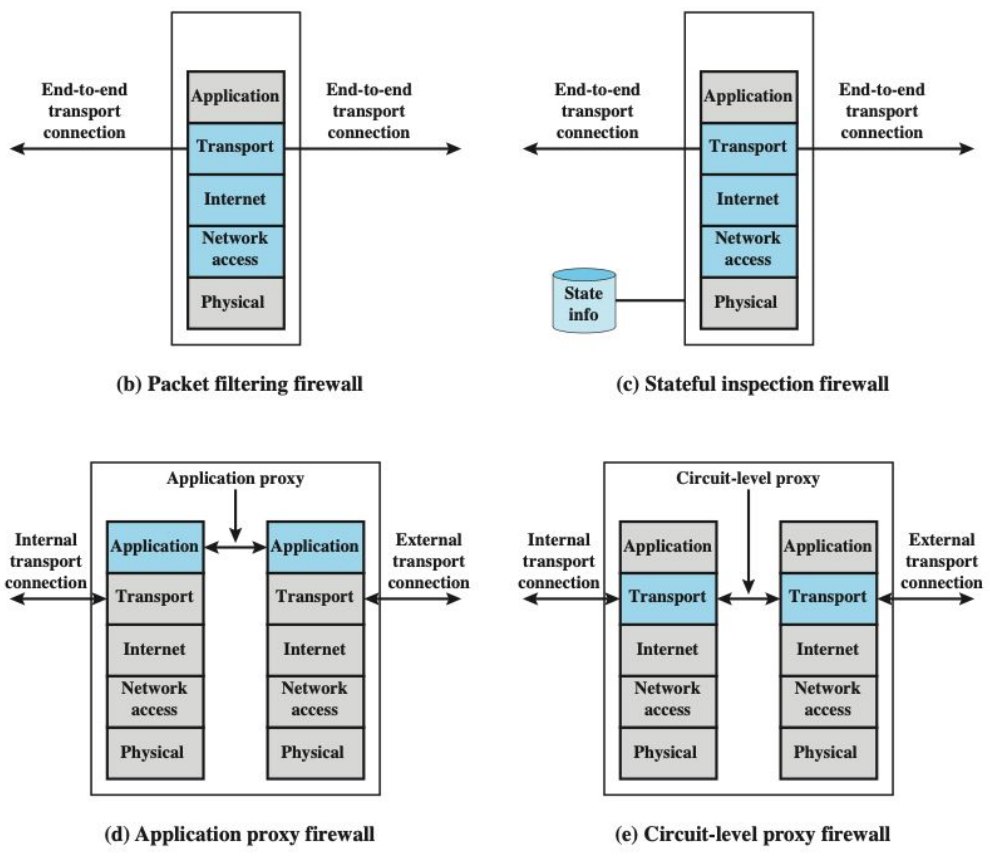
\includegraphics[scale=0.5]{../../immagini/firewall_types}
\end{figure}

\subsubsection{Packet filtering firewall}
Il firewall applica le regole ai pacchetti IP in I/O, solitamente i campi ispezionati da questo di firewall sono
\begin{itemize}
\item IP src/dest address
\item porte src/dest
\item la parte del protocollo IP
\end{itemize}
Solitamente ha 2 policy: discard o accept, possiamo definire black o white list.
\\Vantaggi
\begin{itemize}
\item sono molto semplici
\item trasparenti all'utente
\item molto veloci, possono andare a throughput veloci
\end{itemize}

Svantaggi
\begin{itemize}
\item non possono prevenire attacchi che usano vulnerabilità specifiche dell'applicazione
\item funzionalità di logging limitate
\item non supportano autenticazione utente avanzata
\item vulnerabili ad attacchi che sfruttano bug di TCP/IP
\item una configuazione non corretta può portare a delle brecce
\end{itemize}

\subsubsection{Stateful Inspection Firewall}
L'ispezione è basata sul flusso dei pacchetti
\begin{itemize}
\item se è un flusso TCP, la socket si identifica con le coppie IP,porta src e dest, in più c'è il protocollo
\end{itemize}
I firewall sanno associare lo stato di un pacchetto ad una connessione:
\begin{itemize}
\item se vede un sin, sa che è il primo pacchetto della connessione
\item se vede un altro pacchetto, si salva lo stato in un DB che può essere interrogato per avere informazioni sullo stato della connessione
\item può tenere traccia del sequence number di TCP per prevenire attacchi che si basano su quello
\end{itemize}
Per UDP, non c'è nozione di messaggi di terminazione /inizio, si può usare un timer per considera un flusso UDP concluso ed alcuni firewall avanzati possono andare più in fondo nel protocollo applicativo: in Linux, c'è lo stato related.
\\Se mando una richiesta ICMP e la porta è chiusa, viene mandato un messaggio di port unreachable, il firewall può entrare nei dettagli e capire che il pacchetto è relazionato a quello della richiesta su UDP.
\\Dal punto di vista più semplice c'è una tabella dove ad ogni connessione (IP src/dest e porte src/dest) viene associato lo stato (established etc...)

\subsubsection{Application-level gateway}
Consideriamo un proxy http, per usarlo occorre configurare il browser e nel proxy possiamo forzare delle white list o black list ad esempio per il browsing dei siti web.
\\I firewall sono sicuri, ma non così semplici da configurare, serve il client HTTP per il proxy e deve essere uno per ogni protocollo (applicazione).\\
Questi gateway sono anche detti application proxy, in qaunto agiscono come dei relay per il traffico a livello applicativo:
\begin{itemize}
    \item l'utente contatta il gateway usando un'applicazione TCP/IP
    \item l'utente viene autenticato
    \item il gateway contatta l'applicazione su host remoto e permette l'invio del segmento TCP fra client e server
\end{itemize}
Lo svantaggio più grande è l'overhead addizionale nel processamento dei pacchetti per ogni connessione.

\subsubsection{Circuit level gateway}
Il funzionamento è il seguente:
\begin{itemize}
    \item il gateway mette su due connessioni TCP, una fra se e l'utente sull'host interno e l'altra verso un host esterno
    \item manda i segmenti TCP da una connessione all'altra senza fare ispezione
    \item le funzioni di sicurezza consitono nel determinare quale connessione debba essere permessa. 
\end{itemize}
Usati tipicamente quando l'utente interno è fidato.
\\Il SOCKS v5 proxy è un server che permette di incapsulare diversi protocolli di livello applicativo, progettato per permettere alle applicazioni TCP/UDP di usare in maniera conveniente e sicura un firewall di rete.
\\I client contattano il server SOCKS, si autenticano e mandano le richieste.
\\Il server valuta le richieste ricevute e decide se stabilire la connessione o no.

\subsubsection{Host-Based firewall}
Fin ora abbiamo pensato al firewall come un relay, ma si può implementare anche direttamente sull'host.
\\Può essere utile averli perché il firewall dell'access point non è a grana così fine, mentre quello dell'host può essere configurato a grana più fine, tipicamente l'OS implementa un firewall host-based

\paragraph{Personal-based firewall} Commercialmente sono personal-based firewall, installati nel laptop.
\\Possono essere inseriti in un router che collega tutti PC ad una DSL, ad un modem cablato o ad un'altra interfaccia Internet.
\\Sono tipicamente meno complessi di firewall stand-alone o server-based ed il loro compito principale è negare accesso remoto non autorizzato.
\\Solitamente nei personal firewall ci sono meccanismi per identificare malware

\subsubsection{Approcci e topologie tipiche}
Possiamo avere topologie più o meno complesse, dipendenti dai server, dalle policy da usare etc

\section{NETFILTER}
NETFLITER è un framework che fornisce un hook nel kernel Linux per intercettare e manipolare i pacchetti.
\\I pacchetti che passano per lo stack IP, quindi quelli generati dalla macchina, vengono intercettati, matchati con delle regole specifiche dell'hook ed ogni matching di una regola triggera uno specifico meccanismo, ci sono 5 hooks.
\\Un hook è una callback che viene chiamata nel kernel in base alle esigenze come nel seguente esempio:
\begin{lstlisting}
int ip_local_deliver(struct sk_buff *skb)
{
    struct net *net = dev_net(skb->dev);
    if(ip_is_fragment(ip_hdr(skb))) {
        if(ip_defrag(net, skb, IP_DEFRAG_DELIVER))
            return 0;
    }

    return NF_HOOK(NFPROTO_IPV4, NF_INET_LOCAL_IN,
                   net, NULL, skb, skb->dev, NULL,
                   ip_local_deliver_finish);
}
EXPORT_SYMBOL(ip_local_deliver);

....
int ip_rcv(struct sk_buff *skb, struct net_device *dev, struct packet_type *pt,
           struct net_device *orig_dev)
{
    struct net *net = dev_net(dev);
    skb = ip_rcv_core(skb, net);
    if (skb == NULL)
        return NET_RX_DROP;
    return NF_HOOK(NFPROTO_IPV4, NF_INET_PRE_ROUTING,
                   net, NULL, skb, skb->dev, NULL,
                   ip_rcv_finish);
}
\end{lstlisting}

Tutti i pacchetti intercettati passano per delle tabelle built-in associate agli hook, sono delle linked list.
\\Ogni tabella è dedicata ad una specifica ad un particolare famiglia di azioni
\begin{itemize}
\item filter: inseriamo le regole del firewall, accetta il pacchetto o droppa
\item nat
\item mangle
\item raw: a livello basso, invocata prima della connessione (non la useremo mai)
\end{itemize}
L'immagine di alto livello per i pacchetti generati è la seguente:\\
\begin{figure}[h!]
    \centering
    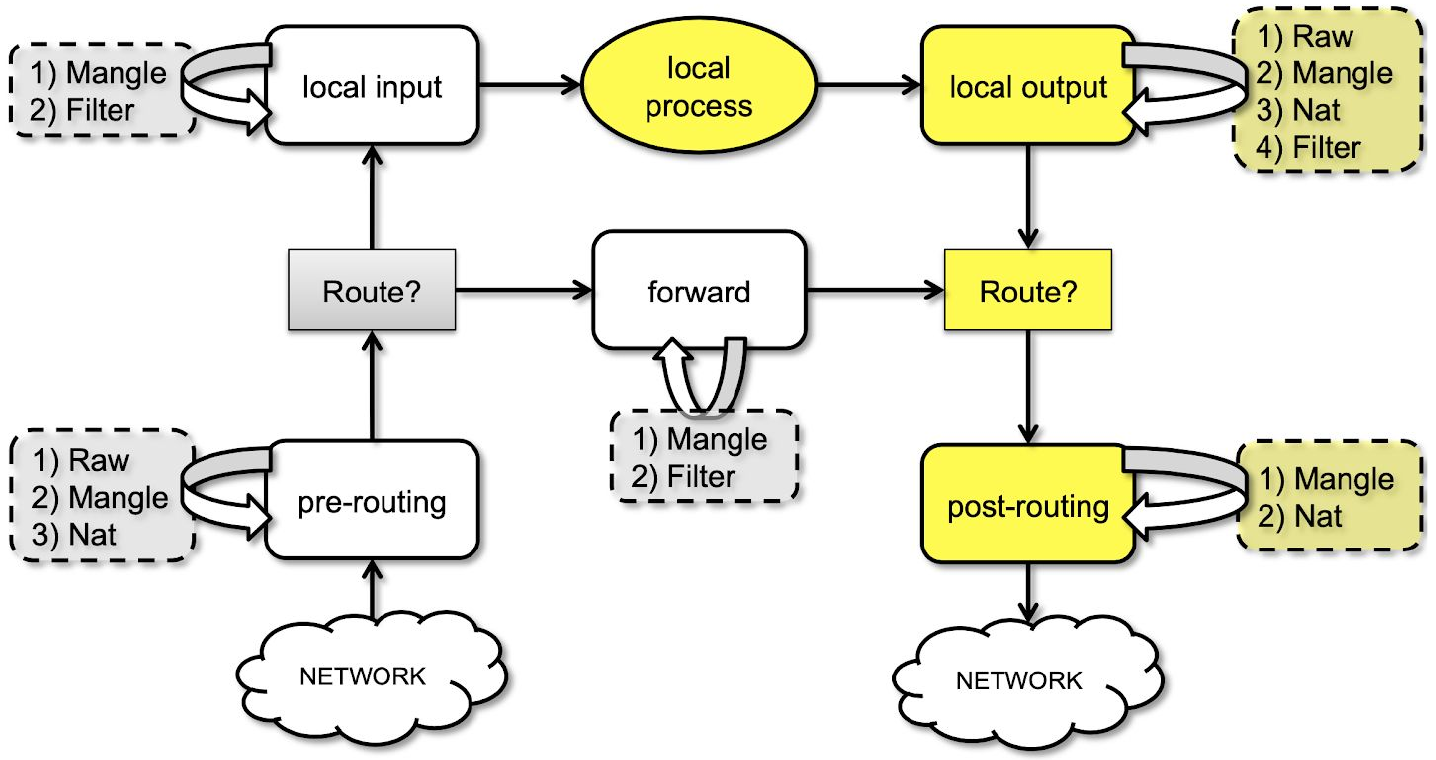
\includegraphics[scale=0.5]{../../immagini/netfilter_lh}
\end{figure}\\\\
nel local output hook ci sono tutte le possibile tabelle built-in, in quanto è possibile anche definire delle tabelle custom, che vengono ispezionate secondo un certo ordine.
\\L'ordine è importante: se viene messa una regola in una tabella che sta sotto nella catena, ed il pacchetto viene droppato prima, non raggiungerà mai la tabella e la regola.
\\Dopo il local, il pacchetto va nel post-routing hook ed alla fine va via.
Per i pacchetti ricevuti verso l'utente:\\ 
\begin{figure}[h!]
    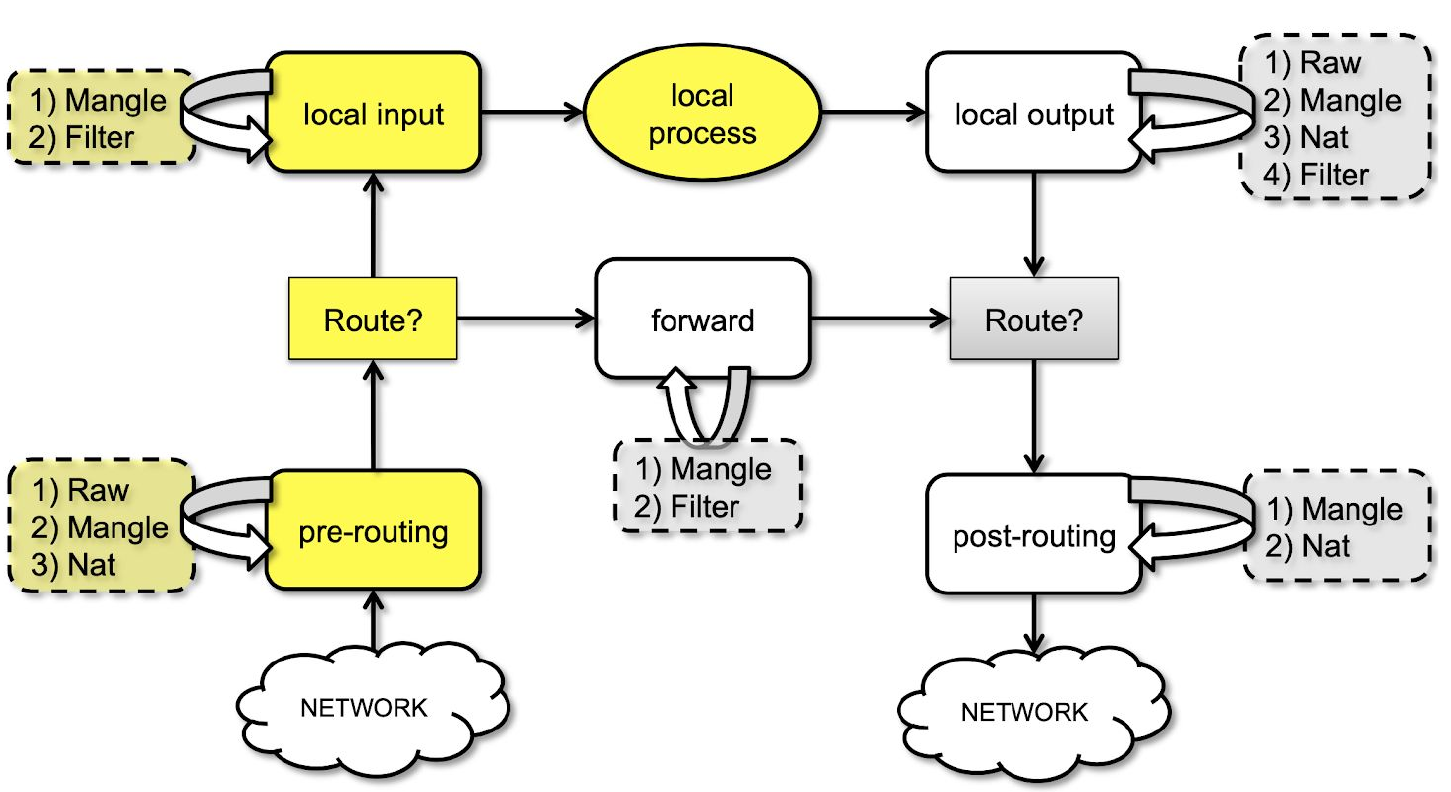
\includegraphics[scale=0.5]{../../immagini/netfilter_recv}
\end{figure}\\\\
nel pre-routing non abbiamo la filter table e dopo il pre-routing sappiamo se il pacchetto è per noi o no.
\\Tracciare lo stato di tutte le connessioni è importante, NETFLITER si appoggia ad un altro modulo del kernel.
\\Con lo stato di match possiamo controllare chi o a cosa è concesso di iniziare una nuova sessione.
\\Lo stato è importante perché ci sono protocolli con stato, come TCP in cui ogni connessione TCP "esegue" una FSM, anche per flussi UDP dove non c'è il concetto di iniziare e chiudere la comunicazione, è possibile capire lo stato dei pacchetti.
Gli stati in cui si può trovare una connessione sono:
\begin{itemize}
    \item NEW
    \item ESTABLISHED
    \item RELATED
    \item INVALID
\end{itemize}

\subsection{ALG related state}
Se estendiamo lo stato al protocollo applicativo, occorre andare nel payload per capire lo stato: quando mandiamo un pacchetto ad una porta chiusa, ad esempio un pacchetto ICMP, otteniamo un messaggio di "port unreachable", quindi c'è lo stato RELATED.
\\In NETFILTER c'è un conntrack helper: ad esempio, nel caso di un'applicazione che usi FTP, si può leggere nel payload il campo di "data port".

\section{iptables}
È il frontend di NETFLITER, usato a user level per configurare una NETLINK socket.
\\iptables viene usato per inserire le regole nelle tabelle, per interagire con NETFILTER.
\\L'API è usata per set uppare, mantenere, ed ispezionare le tabelle con le regole di filtraggio per IPv4 nel kernel Linux, ogni tabella contiene un certo numero di tabelle, ogni tabella ha un certo numero di chain built-in ma anche definite dagli utenti.
\\Una regola del firewall specifica un criterio per un pacchetto ed un target.
\\Se il pacchetto non trova un matching, viene applicata la regola successiva dalla chain.
\\Se il pacchetto non ha alcun match, allora la prossima regola è specificata dal valore del target (opzione -j) che può essere una chain user-defined:
\begin{itemize}
\item ACCEPT
\item DROP
\item QUEUE
\item RETURN
\end{itemize}
I matches di iptables: abbiamo sempre dei match built-in
\begin{itemize}
\item IP source
\item IP dest
\item input interface
\item output interface
\item status
\end{itemize}
ogni match ha delle opzioni proprie, tutti quanti i campi delle opzioni sono in AND logico.

\section*{Lab 006}
Dobbiamo configurare i firewall dopo aver creato la topologia. Andiamo a fare le seguenti cose
\begin{itemize}
\item il firewall sul default gateway per default è accetta tutto. Vogliamo cambiare la policy
\end{itemize}
Con lo state match possiamo fare una cosa del genere:
\begin{itemize}
\item permettiamo tutti i pacchetti dal client al server
\item non ci preoccupiamo più del flusso dei pacchetti da server a client, perché la regola ci dirà che quando i pacchetti sono in stato ESTABLISHED e saranno accettati.
\\Per configurare il firewall sul client, possiamo fare la stessa cosa ma occorre specificare le policy corrette.
\\Nel caso ad esempio della configurazione per le policy di entrata sul default gateway vanno configurate sulla input chain.
\\ IMPORTANTE: per una policy per ICMP, ricordare che questo viene messo direttamente su IP, non è di livello applicativo nel classico stack ISO/OSI, quindi matchamo -P ICMP.
\end{itemize}

\subsection{NAT}
Il NAT è necessario per un ambiente domestico, in una Enterprise magari c'è un range di IP pubblici, ma non li assegniamo a i PC comuni.
\\In Linux, il NAT è implementato sempre da NETFILTER, le regole del NAT interagiscono con quelle del firewall.
\\Cosa possiamo fare con il NAT
\begin{itemize}
\item source NAT, ma se cambia l'IP dell'interfaccia va cambiata a la regola
\item NAT statico
\item redirect locale
\end{itemize}
Il NAT statico setta le regole prima di ricevere il primo pacchetto, mentre il dynamic NAT, fatto con MASQUERADE, viene fatto in modo dinamico: ogni volta che entra un nuovo flusso, viene introdotta una nuova regola nella NAT table.

\section{Packet classification algorithms and data structures}
Perché la classificazione dei pacchetti è così importante: è un operazione fondamentale non richiesta solo dai firewall, abbiamo visto come configurare i firewall.
\\Un algoritmo di PC veloce è un building block fondamentale dei firewall, ma anche in altri campi dell'ingegneria del traffico e delle TLC.
\\Sappiamo che il packet forwarding basato su longest prefix matching è conosciuto, LPM può essere visto come un algoritmo specifico di packet classification.
\\Abbiamo diversi approcci per implementare LPM, come ad esempio il seguente\\
\begin{figure}[h!]
    \centering
    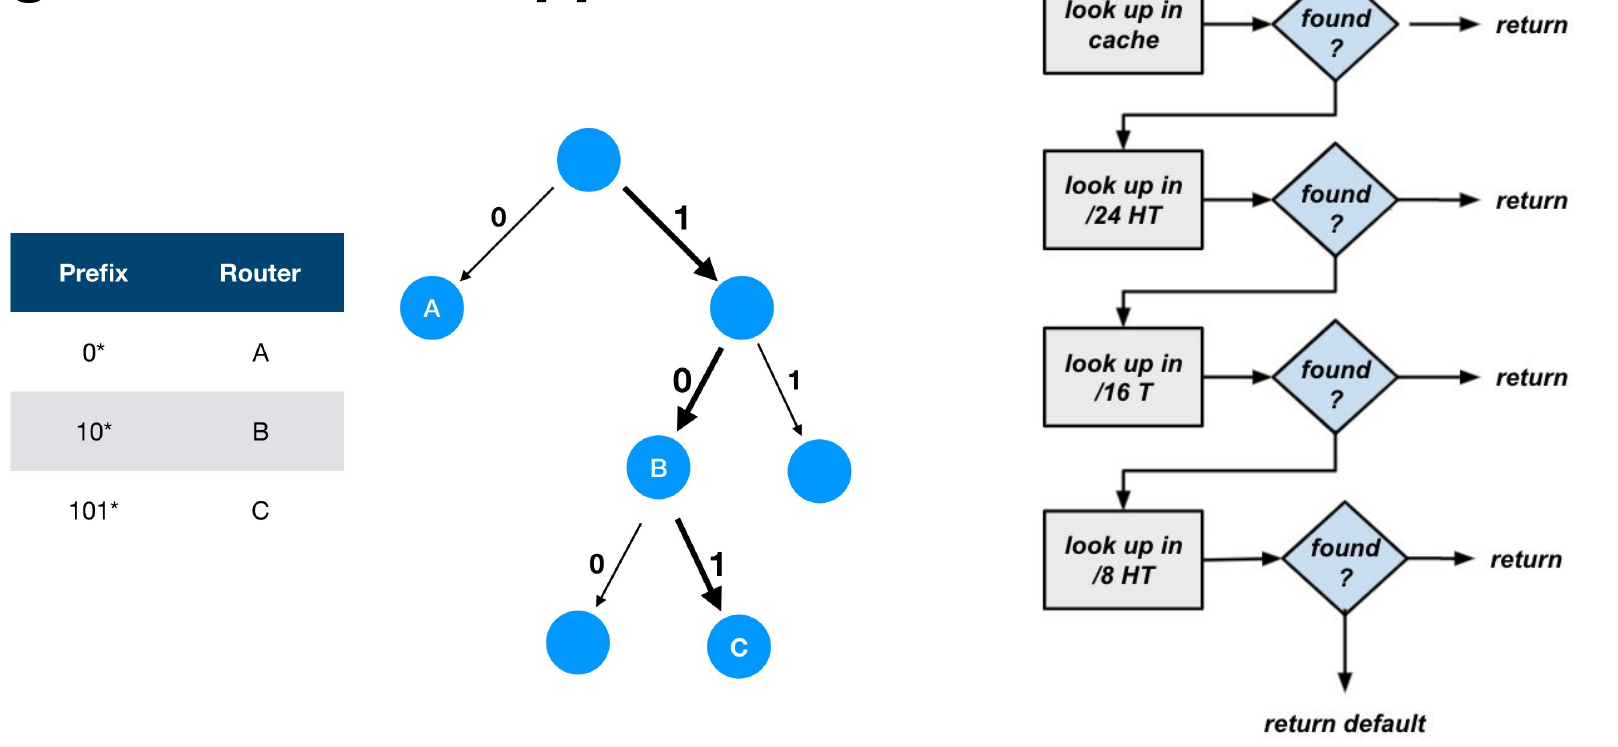
\includegraphics[scale=0.45]{../../immagini/lpm_ex}
\end{figure}\\\\
Abbiamo però bisogno di algoritmi diversi per use case diversi, vista l'evoluzione continua dell'Internet

\subsection{Problema del packet classification}
La classificazione avviene facendo il matching con delle specifiche regole, il problema è trovare la regola di costo più basso che matchi il messaggio in input.
\\L'informazione di un lookup è contenuta in K diversi header field, gli header sono denotati con H[i].
\\Il classificatore consiste in un insieme di regole $R_i$ ed ogni campo in una regola può avere 3 match
\begin{itemize}
\item exact match, come ad esempio il look-up del MAC, cerchiamo proprio quel MAC
\item prefix match, quindi come LPM
\item range match, ovvero ad esempio droppare tutti i pacchetti tcp da porta 1000 a 2000
\end{itemize}
Ogni regola è associata ad una direttiva che dice come processare il pacchetto che matcha la regola.
\\Un pacchetto P matcha la regola R se ogni campo di P matcha il corrispondente campo di R, e questa corrispondenza è implicita nella specifica del campo:
\begin{itemize}
    \item se la destinazione è specificata come 1010*, allora richiede prefix matching
    \item se il protocollo è UDP, richiede exact matching
    \item se il campo della porta è un range, come 1024-1100, allora è richiesto un range match 
\end{itemize}
Per esempio, se abbiamo la regola\\ 
\textbf{R = (100*, *, TCP, 1024:1080, *)} [ip src (in bit), ip dest (in bit), protocol, port range, ..]con \textbf{disp=DROP};
\\ogni wildcard dice che si matcha qualsiasi cosa.
\\Siccome ogni pacchetto può corrispondere a diverse regole nel database, ogni regola ha un costo non negativo \textbf{cost(R)}, l'ambiguità viene risolta ritornando sempre la regola col costo minimo e l'obiettivo è quello di ritornare la prima regola meno costosa.

\subsection{Requisiti e metriche}
I requisiti del matching sono simili a quelli del lookup di IP, vorremmo poter fare classificazione dei pacchetti alla velocità del cavo per i pacchetti di taglia minima, ma anche di ridurre la quantità di memoria usata.
\\Dipende ovviamente dallo scenario, magari abbiamo dell'hardware dedicato che implementa delle tabelle che vengono controllate veloci ma c'è poca memoria etc...
\\Per la maggior parte dei database dei firewall, la velocità di inserimento non è un problema perché le regole vengono cambiate di rado, una volta settate all'inizio rimangono così.
\\Non è sempre vero, ad esempio NETFILTER usa un firewall statefull, quindi serve anche fare le insert nel DB velocemente.
\\Quindi se vogliamo anche insert veloci abbiamo una 3 metrica, che è il fast update time.
\\Abbiamo visto iptables, perché è una implementazione di firewall statefull molto noto, è stata molto usata perché flessibile ma ha problemi di velocità e scalabilità: il problema è l'algoritmo di classificazione, che è lineare ovvero O(N), se abbiamo N regole si fanno N lookups.
\\Ma non è la sola ragione, l'altra è che NETFILTER è molto interconnessa con il resto del modulo di networking di Linux, quindi c'è molto overhead dovuto all'interazione.
\subsubsection{Possibili soluzioni}
Una possibile soluzione potrebbe essere il caching della ricerca fatta per il primo pacchetto accoppiata all'intero header.
\\Il rate delle cache hit è al più sul 80/90\% ma in realtà è più basso, quindi il 10\% delle volte si prende la strada più lenta e nel caso peggiore.
\\ Considerando ad esempio che la ricerca in una cache richieda 100nsec e che una ricerca lineare di 10000 regole costi 1.000.000 ns, quindi 1msec, abbiamo quindi 0.1 msec di tempo di processamento con un hit rate del 90\% che non va comunque bene.\\\\
Soluzione migliore: una CAM è una memoria dove la prima cella che corrisponde un dato verrà restituita usando un lookup parallelo su hardware.
\\Un CAM ternario permette ad ogni bit di dati di essere 0 o 1 o una wildcard, ma ci sono comunque diverse alternative al considerare tCAMs, tra cui il fatto che comunque serve dell'hardware dedicato:
\begin{itemize}
    \item CAM a densità minore e potenza maggiore rispetto ad SRAM
    \item difficoltà di integrazione delle logiche di forwarding con le CAM
    \item moltiplicazione delle regole causata dai range
    \item molteplici produttoridi CAM hanno anche considerato soluzioni algoritmiche
\end{itemize}
Questo è il modo di funzionamento di un tCAM\\
\begin{figure}[h!]
    \centering
    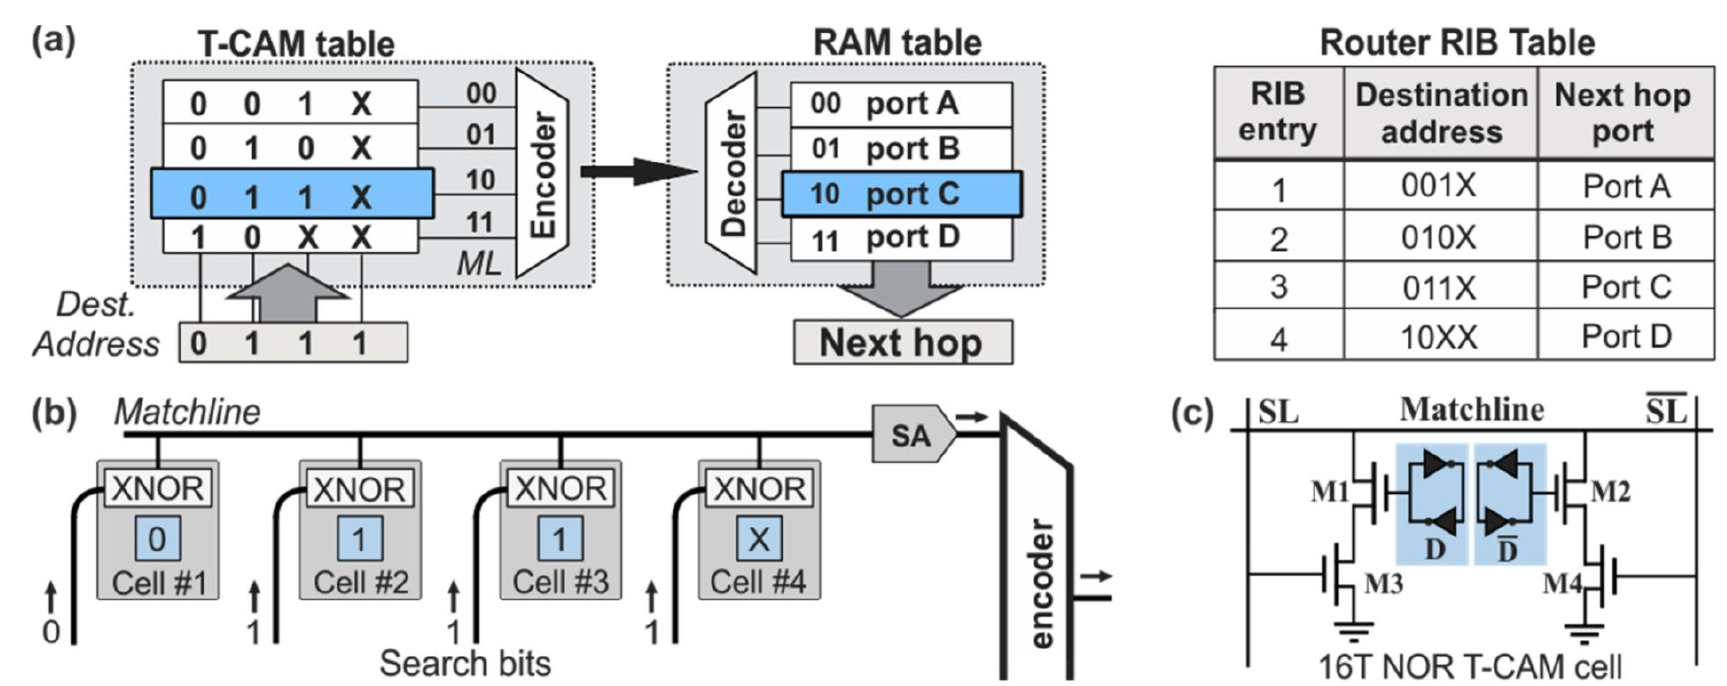
\includegraphics[scale=0.5]{../../immagini/tcam}
\end{figure}

\subsection{Schema uni-dimensionale}
Il blocco fondamentale è il \textbf{prefix tree}, un albero usato per localizzare le chiavi, nell'esempio cerchiamo la chiave "ted", ma anche "teddy" sarebbe arrivato lì perché era il prefisso più lungo:\\
\begin{figure}[h!]
    \centering
    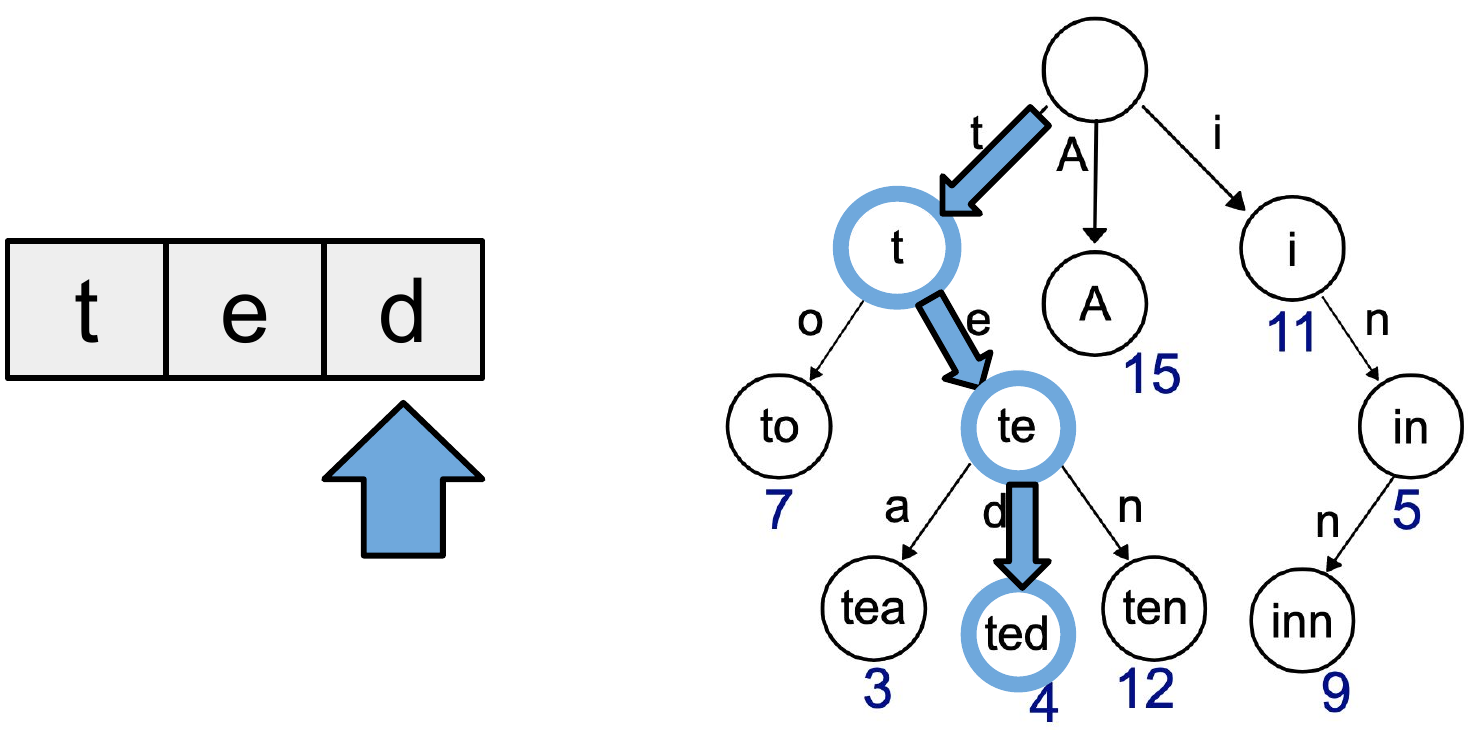
\includegraphics[scale=0.5]{../../immagini/tries}
\end{figure}\\\\
Consideriamo di avere un database dei prefissi di referenza: non ci preoccupiamo dell'azione associata, ma solo del match.
\\Vogliamo cercare il prefisso più lungo che corrisponde ad un indirizzo

\subsubsection{Unibit tries}
La prima idea è quella di creare un prefix trie, ottenendo una struttura del genere:\\
\begin{figure}[h!]
    \centering
    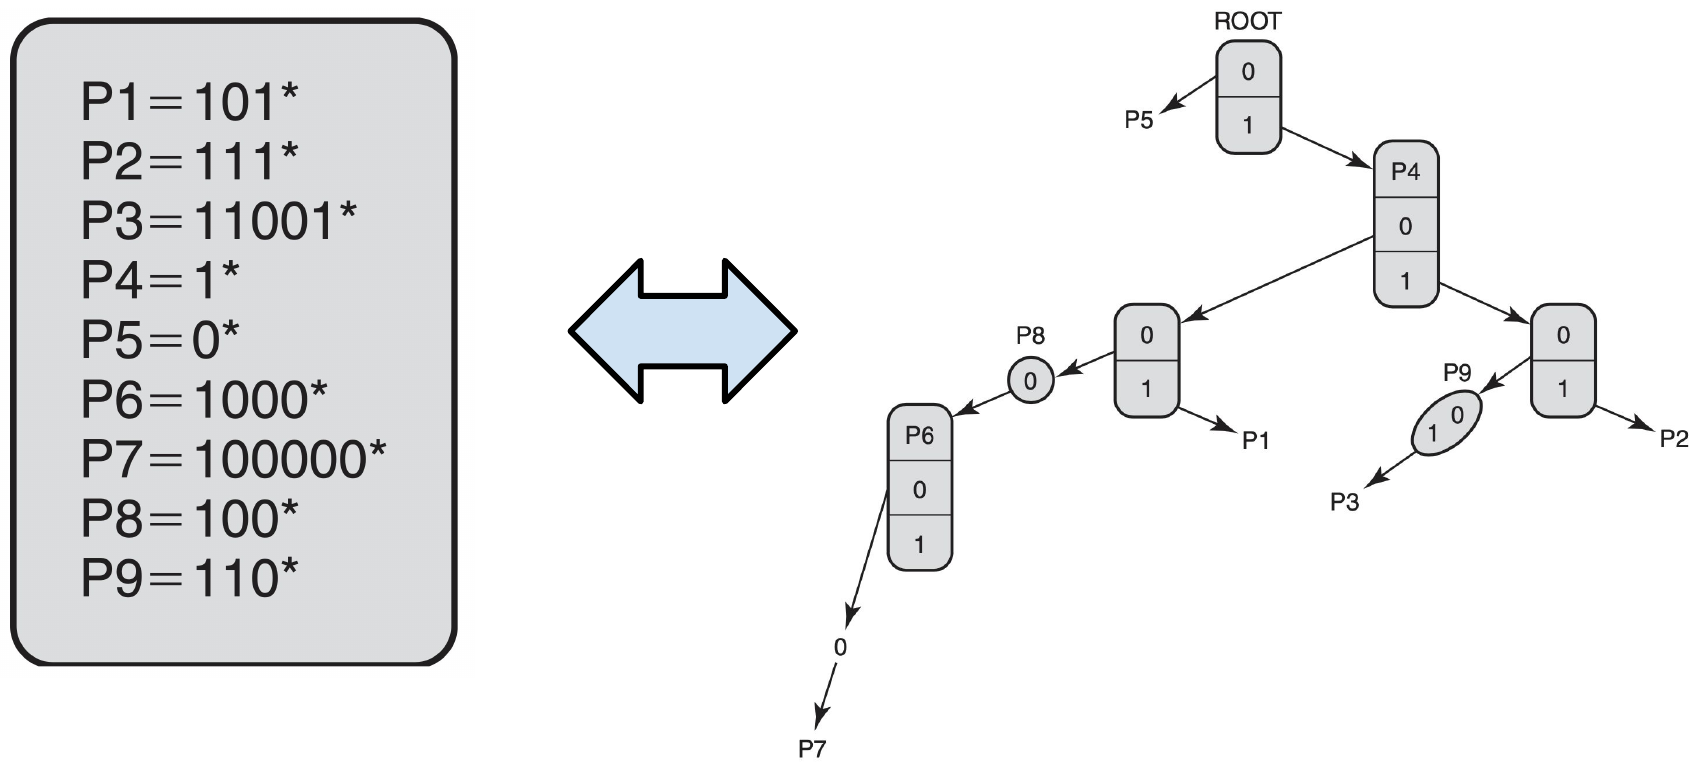
\includegraphics[scale=0.5]{../../immagini/unibit_tries}
\end{figure}\\\\
per fare il lookup della chiave, prendiamo i bit che la compongono, quindi viene estratto il dest address dal pacchetto e viene scorso bit a bit, ed ogni volta aggiorno quale è il longest prefix che ho incontrato scendendo nell'albero.
\\Ci sono diversi lookups, nel caso di IPv4 facciamo al più 32 lookup, mentre nel caso IPv6 128 e le memorie per lo più usate sono le DRAM, quindi più lente.
\\Quindi, questo motiva la multibit trie search

\subsubsection{Multibit tries}
I nodi possono avere più bit associati, dobbiamo scegliere quanti bit avere in ogni nodo ma sopratutto se avere un numero fissato di bit o variabile.
\\Decidiamo di scegliere 3 bit per ogni nodo, dobbiamo implementare la controlled expansion: il problema è che ci può essere una collisione, ad esempio data dall'espansione di P6 con P7:\\
\begin{figure}[h!]
    \centering
    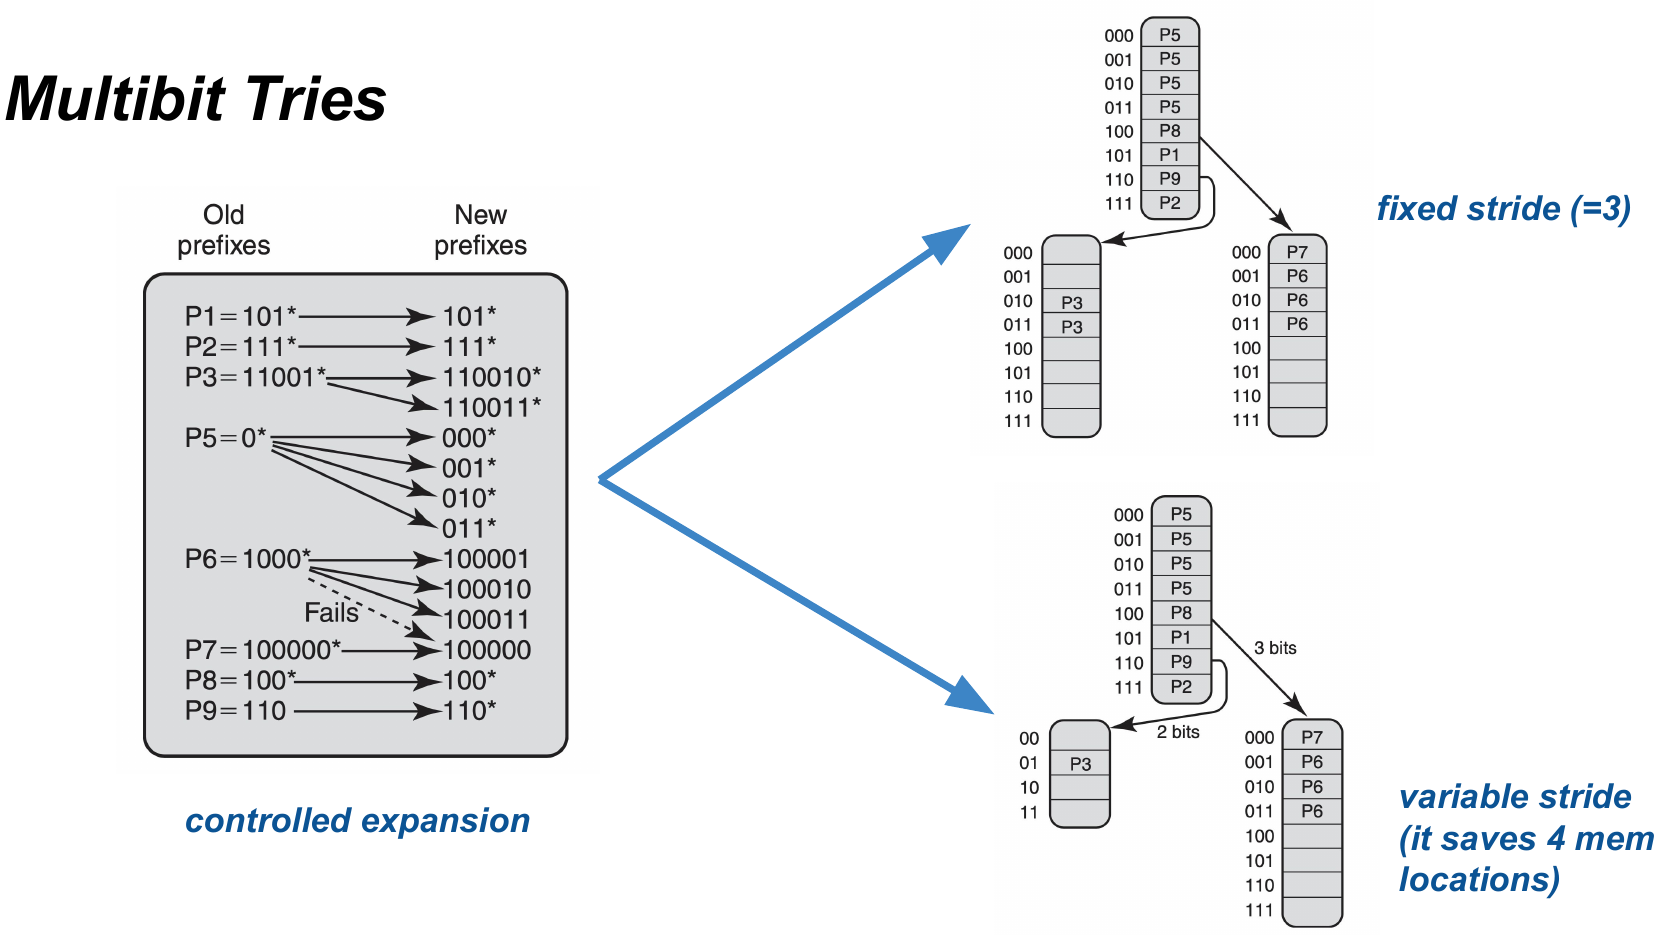
\includegraphics[scale=0.5]{../../immagini/multibit_tries}
\end{figure}\\\\
il problema è che un albero fissato può portare a dello spreco di memoria.\\
Il problema di scegliere uno stride ottimo non è triviale, ci sono diversi approcci.
\\Possiamo comunque fare di meglio, in quanto stiamo comunque sprecando della memoria.

\subsubsection{LC tries}
La cosa fondamentale da ricordare è che il LPM è un caso particolare di algoritmo di classificazione di tipo prefix, la soluzione più nota è l'LC tries\\
\begin{figure}
    \centering
    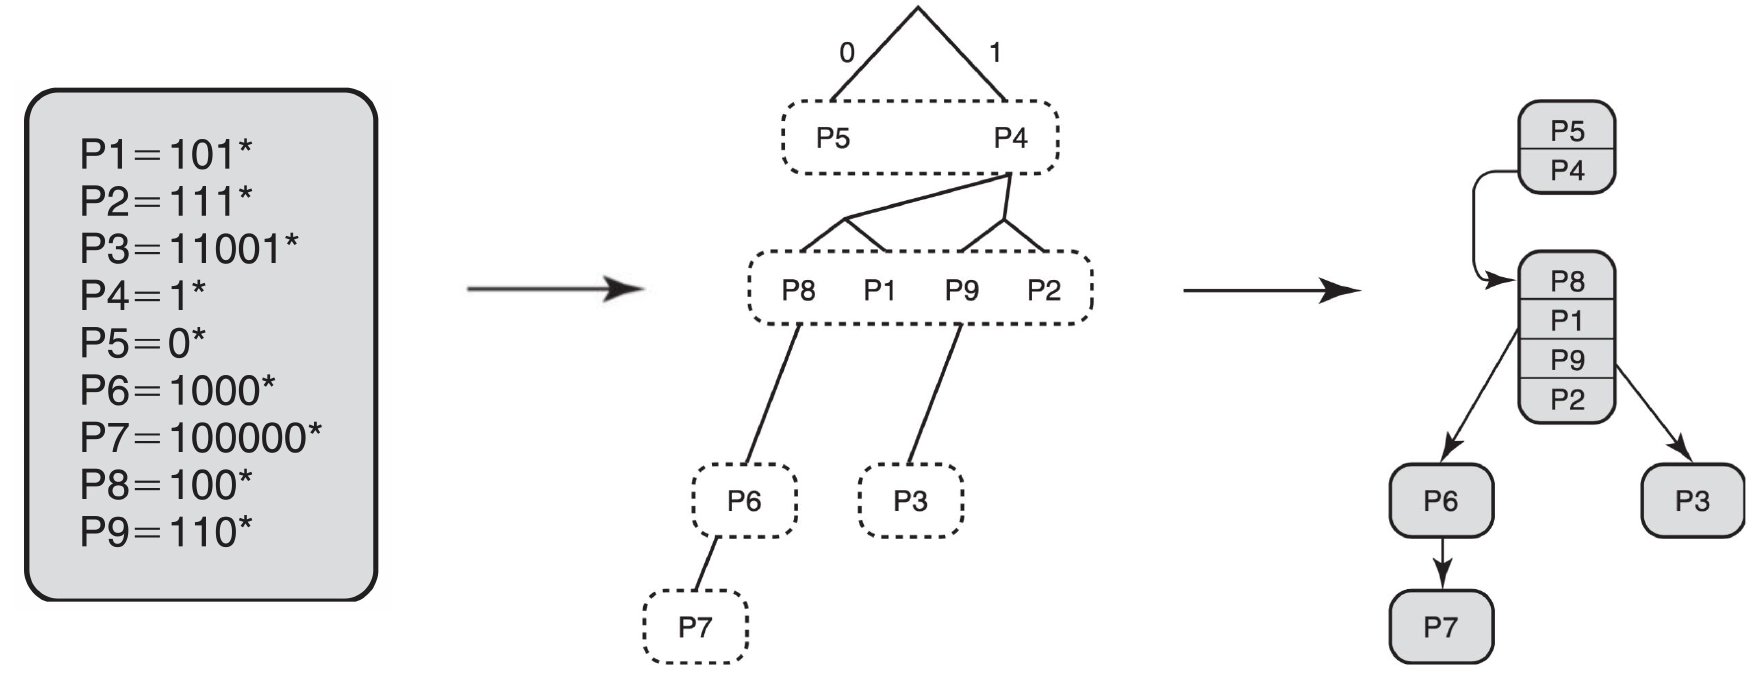
\includegraphics[scale=0.5]{../../immagini/lc_trie}
\end{figure}

\subsection{Algoritmo generalizzato per matching esatto}
In alcuni casi, lavora bene la soluzione di exact matching, come ad esempio la ricerca binaria che è una ricerca di tipo esatto.
\\Un'altra generalizzazione è quella dell'hash table, usando una pipeline per fare prefix matching

\subsubsection{Binary search}
Nella ricerca binaria su range, ogni prefisso è rappresentato con un range, usando l'inizio e la fine del range: ad esempio, il prefisso 10** mappa sul range da 1000 ad 1011.
\\Gli endpoint dei range di N prefissi partizionano lo spazio degli indirizzi in 2N+1 intervalli disgiunti.
\\Come costruiamo un albero o tabella di ricerca binaria: abbiamo gli end points dei nostri range
\begin{itemize}
\item P4: 1***
\item P1: 101*
\end{itemize}
abbiamo 2 prefissi
\begin{itemize}
\item nella prima colonna, abbiamo indirizzi che sono strettamente maggiori dell'end point e sono più piccoli del valore successivo in tabella
\item sulla seconda colonna, abbiamo indirizzi che corrispondono esattamente all'end point
\end{itemize}
quindi abbiamo la seguente tabella, che al più 2N entry, e può essere attraversata in tempo logaritmico\\
\begin{figure}[h!]
    \centering
    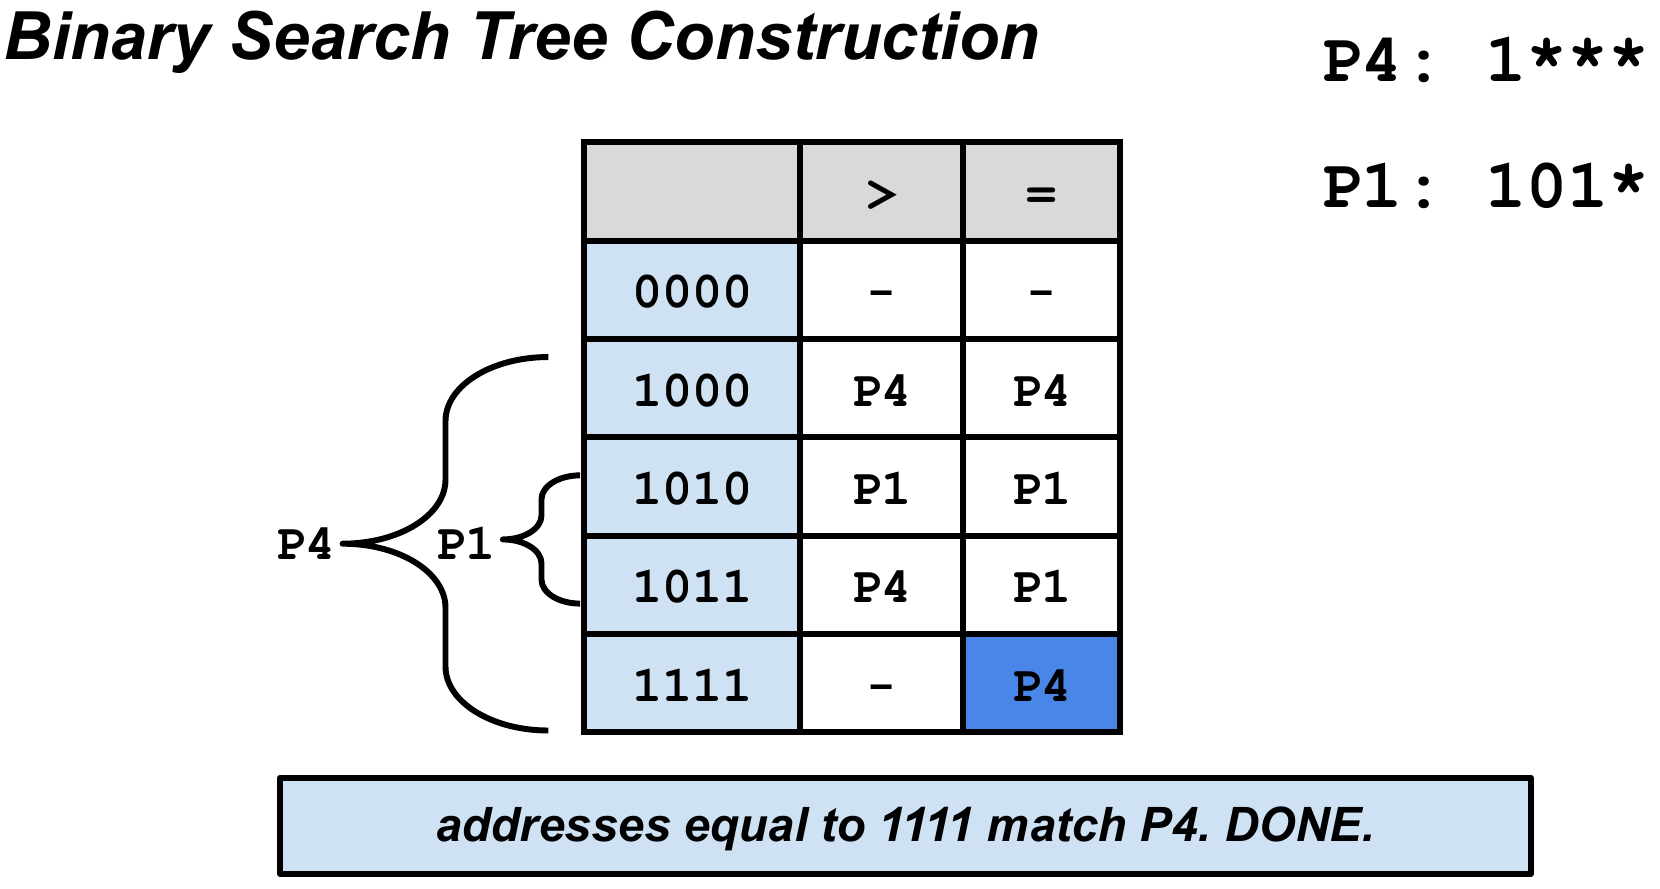
\includegraphics[scale=0.5]{../../immagini/bst}
\end{figure}

\subsubsection{Hashing exact match}
Come fare LPM con hash tables, dobbiamo considerare più hash table che devono essere tante quante il più lungo prefisso, quindi in totale 32 per IPv4.
\\Quindi, nell'esempio del DB, dividiamo in 4 hash table, mettendo i prefissi in ordine decrescente di prefissi.
\\I problemi delle hash tables: se facciamo una hash table, se il result set è più piccolo del set di partenza, ci sono collisioni e per risolverlo si può usare ad esempio una lista collegata, che va scorsa per trovare il record corretto.
\\Ci sono anche problemi sul dimensionamento e sul resize.
\\Abbiamo le diverse hash tables, assumiamo di fare il lookup di 0101:\\ 
\textbf{Approccio lineare:}\\
l'approccio base è fare una ricerca lineare\\
\begin{figure}[h!]
    \centering
    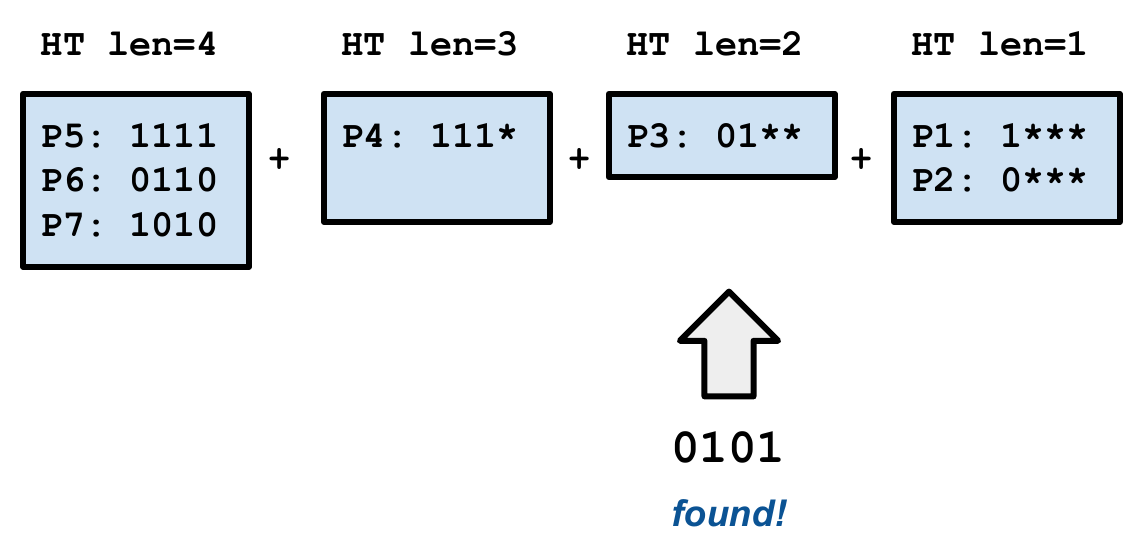
\includegraphics[scale=0.5]{../../immagini/linear_search}
\end{figure}\\\\
nel caso di una wildcard, mettiamo in AND i bit con la wildcard con quelli della chiave cercata.\\
\textbf{Binary search:}\\
costruiamo un albero binario\\
\begin{figure}[h!]
    \centering
    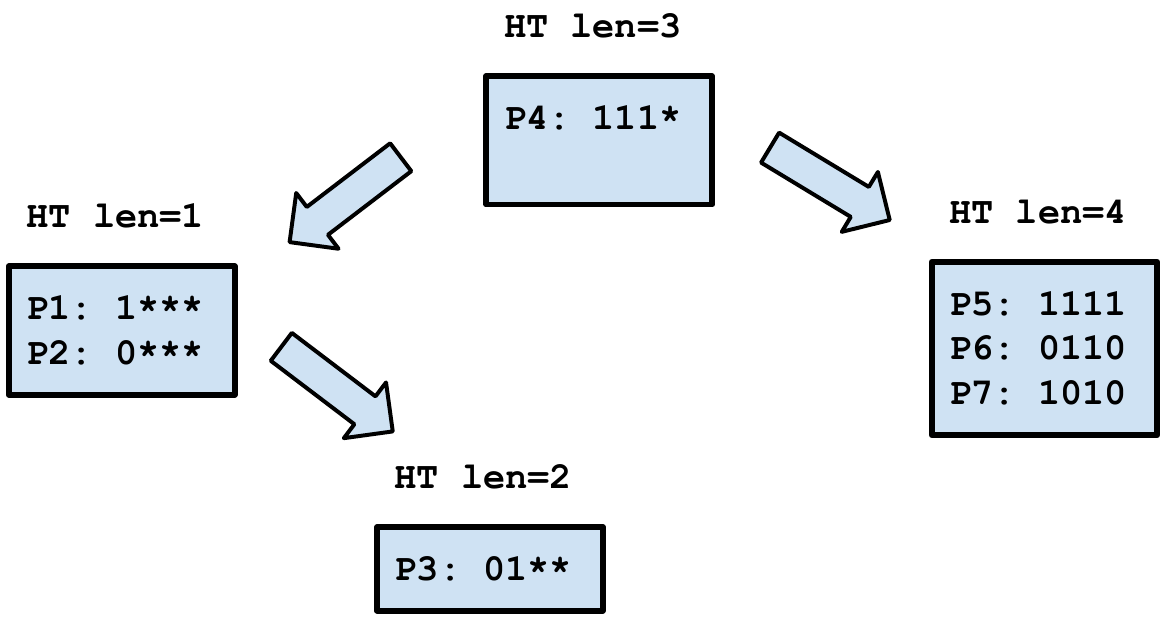
\includegraphics[scale=0.5]{../../immagini/ht_search}
\end{figure}\\\\
se trovo un match, vado a destra e se non lo trovo a sinistra.
\\Ma c'è un problema: se non ho un match, non vuol dire che non posso trovare un prefisso a destra, quindi l'approccio è greedy e serve un match artificiale detto \textbf{marker} quando c'è un potenziale prefisso più lungo che corrisponde:
\begin{itemize}
\item ho due marker nella prima tabella, se ho un match non vuol dire che ho trovato la key giusta
\item vado a destra e trovo il match
\end{itemize}
ma anche qui c'è lo stesso problema di prima, ovvero rischio di prendere la scelta sbagliata.
\\La soluzione è best prefix match, ovvero a setup time pre-computiamo un insieme di bmp:\\
\begin{figure}[h!]
    \centering
    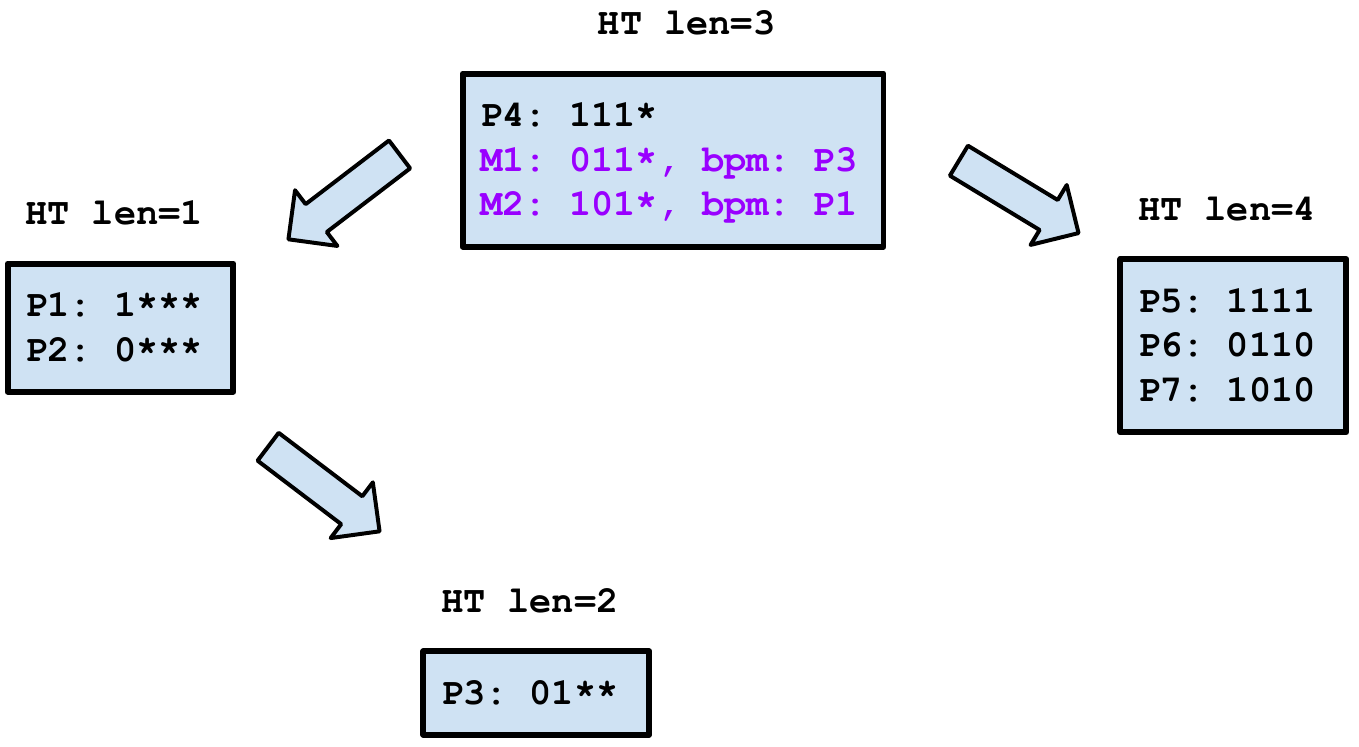
\includegraphics[scale=0.5]{../../immagini/bpf}
\end{figure}

\subsection{Schema bi-dimensionale}
La classificazione dei pacchetti è un problema più generale, partiamo col definire degli schemi efficienti quando ci sono due dimensioni, ovvero basandosi su una combinazione arbitraria di due campi, ad esempio la combinazione di IP src e dest.
\\Il DB delle regole di riferimento è il seguente:\\
\begin{figure}[h!]
    \centering
    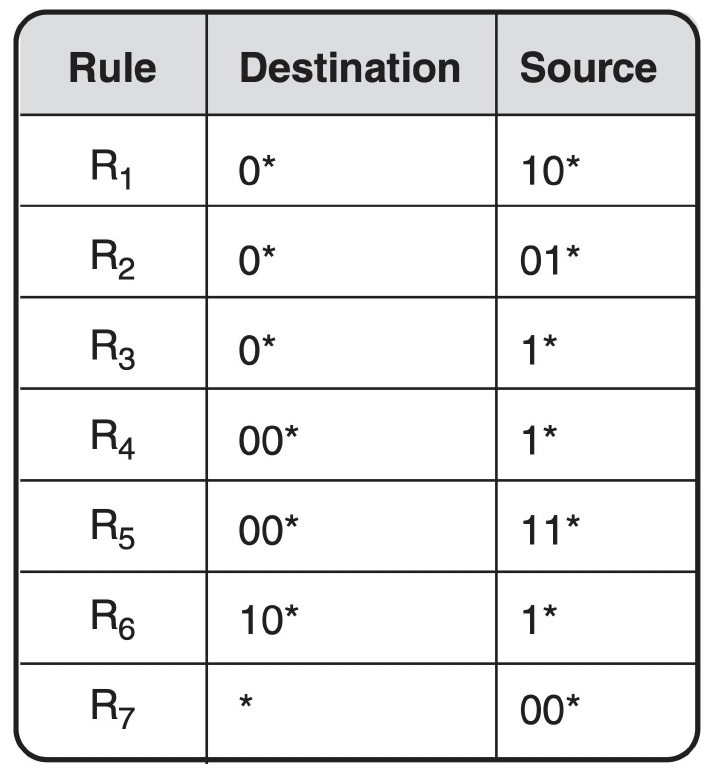
\includegraphics[scale=0.5]{../../immagini/2dim_db}
\end{figure}\\\\
dest e scr sono dei casi speciali di matching di wildcard, se matchiamo la regola 4, potremo anche prendere la regola 1, ma dipende tutto dalla priorità che diamo alle regole.
\\Per poter risolvere il problema, siamo partiti dallo schema uni-dimensionale, quindi abbiamo diversi approcci.
\subsubsection{Set-Pruning Tries}
Creiamo un prefix tree per il campo destinazione, ed appendiamo a ciascuno prefissi dell'albero un insieme di sotto-tries che rappresentano le sources che matchano con la regola.
\\Quali sono i prefissi delle source da mettere nei tries dipende dal DB:\\
\begin{figure}[h!]
    \centering
    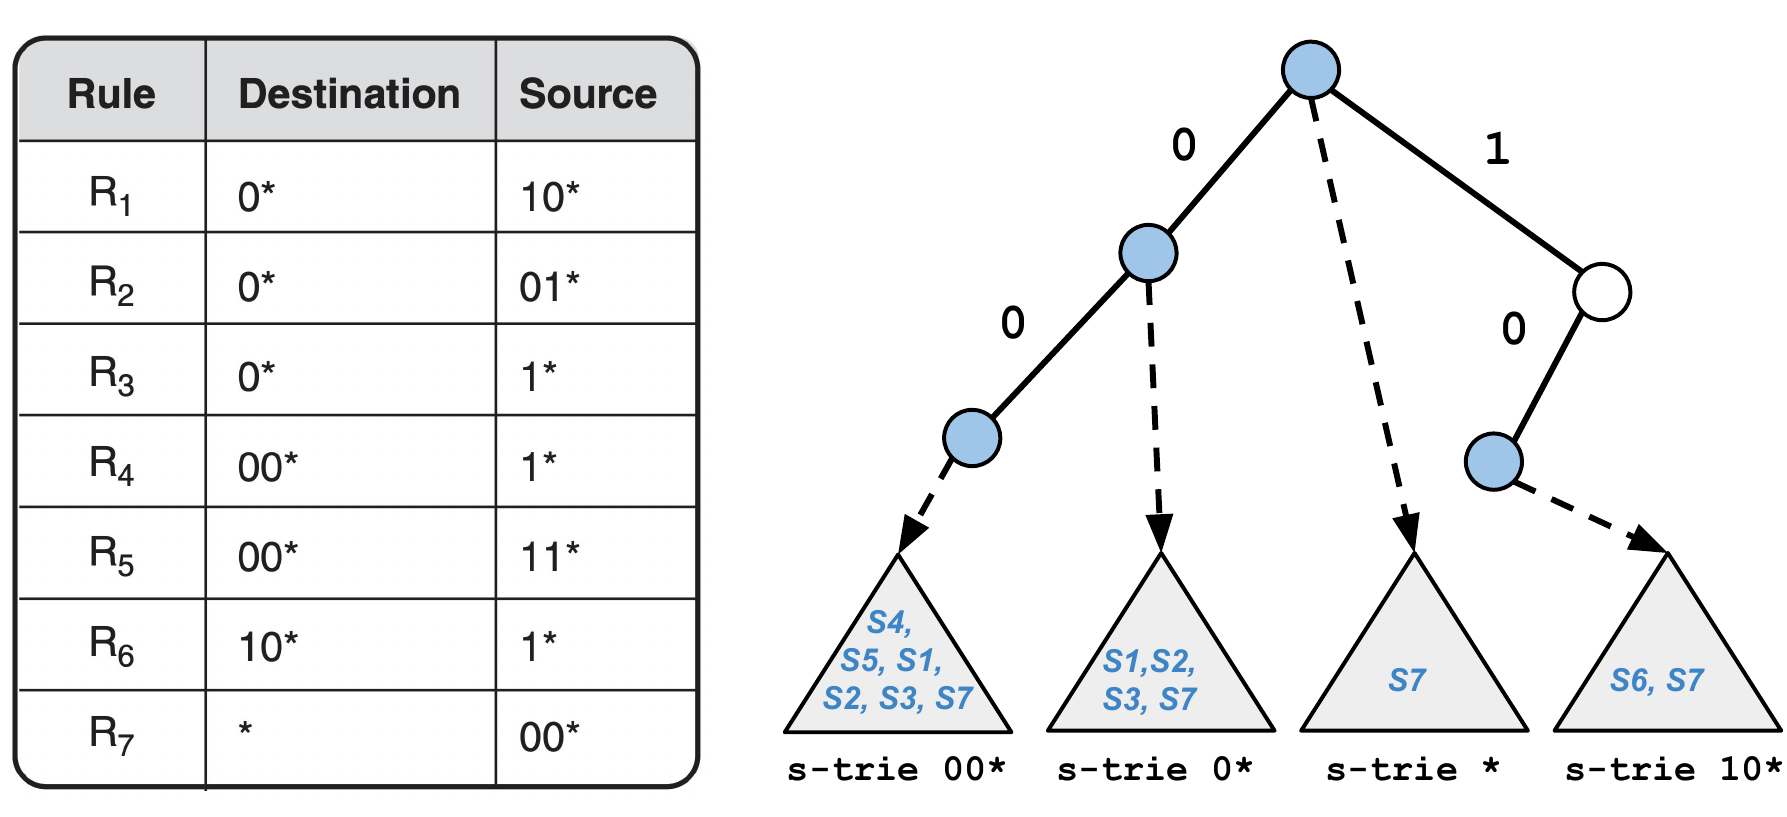
\includegraphics[scale=0.5]{../../immagini/sp_tries}
\end{figure}\\\\
in termini di memoria, si spreca molto perché molti prefissi vanno in più sotto-tries.
\\Se quindi abbiamo dei source tries che sono esattamente gli stessi non li replichiamo, che è la prima ottimizzazione ovvia da fare, ma serve qualcosa in più.
\subsubsection{Backtracking look up}
È possibile applicare una strategia di back tracing, dove non si replicano i prefissi che sono inclusi nel sotto-prefisso di una destinazione.
\\Ad esempio nel nodo a sinistra, abbiamo un antenato del prefisso che lo contiene, quindi non occorre replicarlo\\
L'algoritmo di ricerca procede per back searching, procedendo come in figura\\
\begin{figure}[h!]
    \centering
    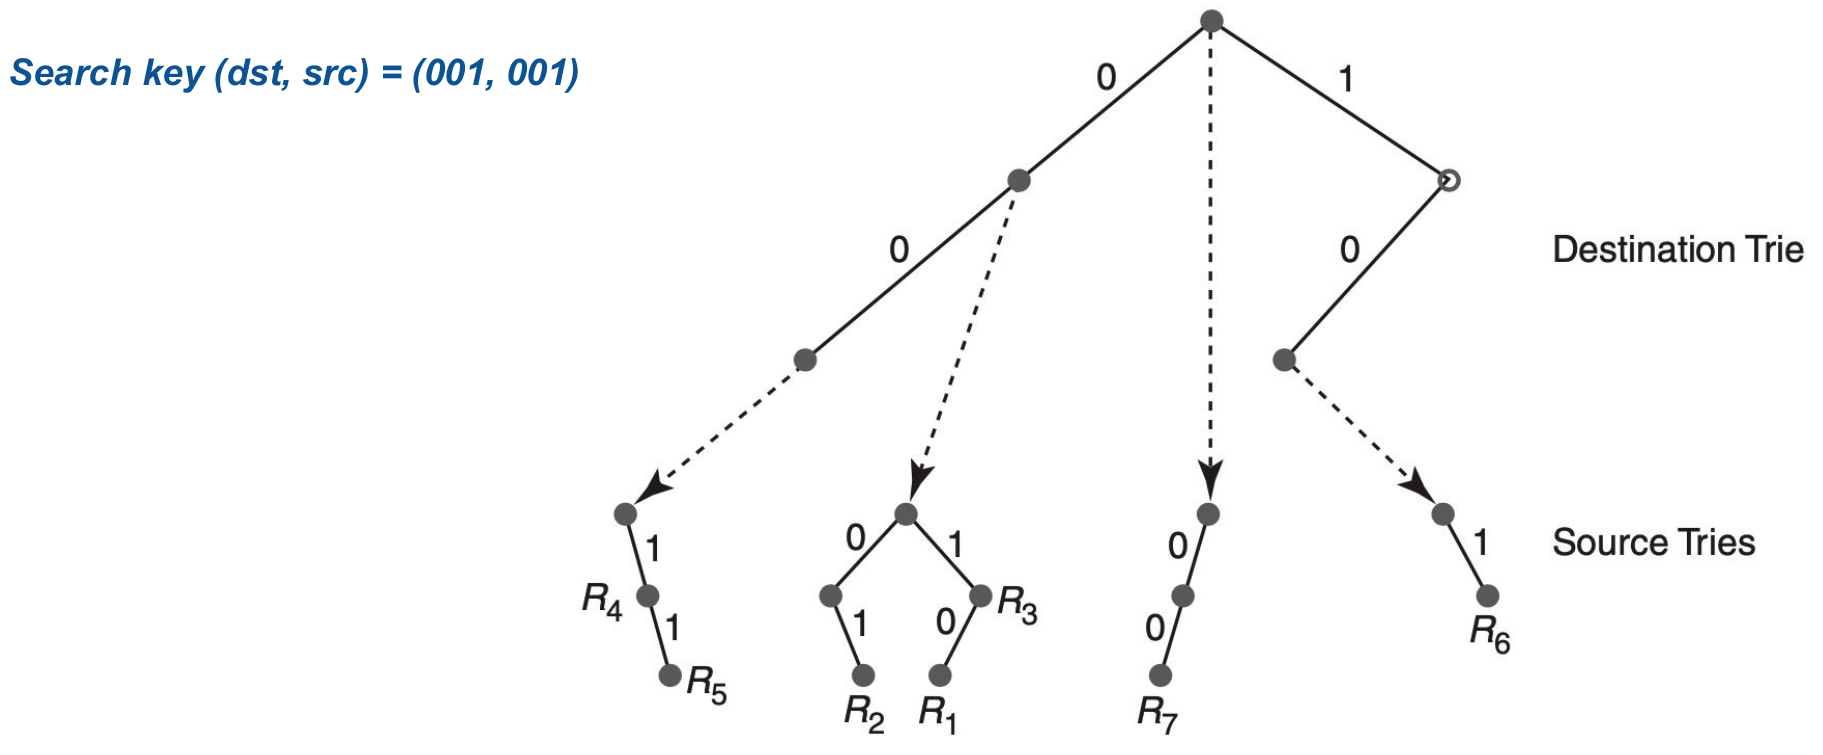
\includegraphics[scale=0.5]{../../immagini/backtracking}
\end{figure}\\\\
attraversiamo l'albero per cercare il longest prefix matching nel dest field dell'header.
\\Ora dobbiamo cercare il matching nel sotto-albero: dobbiamo fare back tracing, fino ad un prefisso che matcha il dest field e quindi andare a vedere se c'è un matching nel src, se troviamo un matching si aggiorna la regola di matching trovata.
\\Diventa una ricerca lineare, ma i src prefixes sono solo in un sotto-albero ma c'è un spreco perché sappiamo già quando non c'è un matching.

\subsubsection{Grid of tries}
Si può introdurre uno switch pointer, ovvero un puntatore ad un nodo da cui possiamo far ripartire la ricerca in caso di non matching.
\\Ora abbiamo una griglia di puntatori che dicono da dove ripartire che vanno precomputati.
\\Dall'esempio, abbiamo anche un problema perché tutto funziona solo se la priorità è intrinseca nel fatto che si prende il prefisso più lungo, ma se cambiasse la regola di priorità non funzionerebbe più.
\\Quindi, anche se abbiamo il matching su una specifica regola, aggiungiamo qual è la regola che effettivamente matcha, anche questi valori vengono pre-computati.
\\È il miglior approccio per uno schema bi-dimensionale, ma c'è un problema: chi implementa questo tipo di policy di filtraggio non controlla solo due campi ma verosimilmente molti ed usando un approccio del genere si ha una taglia dello storage che cresce esponenzialmente.
\\Ma in pratica, i veri DB sono strutturati e questa struttura può essere sfruttata per risolvere il problema della classificazione con tecniche algoritmiche.

\subsubsection{Estensione dello schema bi-dimensionale}
La classificazione dei pacchetti si può derivare da un insieme di database di firewall osservati:
\begin{itemize}
    \item il prefix containment è raro. È raro quindi avere prefissi che sono prefissi di altri prefissi
    \item molti campi generalmente non sono range
    \item il numero di regioni di classificazione disgiunte è piccolo
    \item quasi tutti i pacchetti matchano al più 5 disinti valori src-dest
\end{itemize}
Come è  possibile quindi implementare uno schema multi-dimensionale:
\\La prima idea non naive si basa sul punto 4: creiamo una grid of tries dove connettiamo alla parte finale dell'albero una lista lineare di regole.
\\Questo funziona se non si hanno molte regole, ma in generale non è così.
\\Ci sono dei casi in cui è richiesto di avere soluzioni migliori.
\\\\Abbiamo quindi l'idea del divide et impera: spezziamo il problema in sotto-problemi
\begin{itemize}
\item cominciamo con lo spezzare il DB delle regole in colonne, dove ogni colonna è uno "sliced" DB (vedi immagine)
\item dato un pacchetto P, determiniamo i prefissi che matchano per ognuno dei suoi campi separatamente
\item infine, si combinano i risultati dei lookup sul best-matching prefix sui campi individuali
\end{itemize}
Ci sono 3 metodi per realizzare l'algoritmo
\begin{itemize}
    \item bit vector linear search
    \item Cross-Producting
    \item decision tree approach
\end{itemize}
Questo è il DB che consideriamo per gli esempi, con la seguente topologia:\\
\begin{figure}[h!]
    \centering
    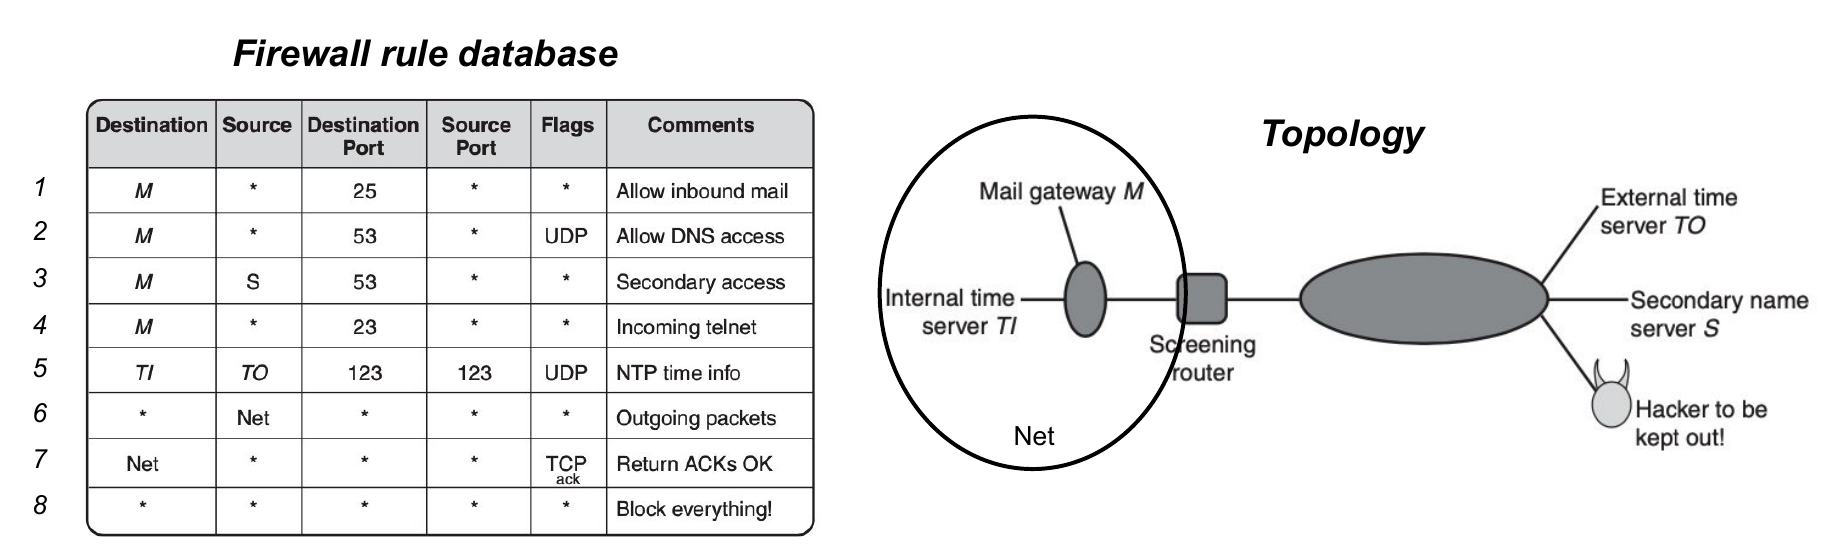
\includegraphics[scale=0.5]{../../immagini/bidim_topology}
\end{figure}\\\\

\paragraph{Bit vector linear search:} Abbiamo un vettore di bit con un 1 in corrispondenza delle regole che matchamo:\\
\begin{figure}[h!]
    \centering
    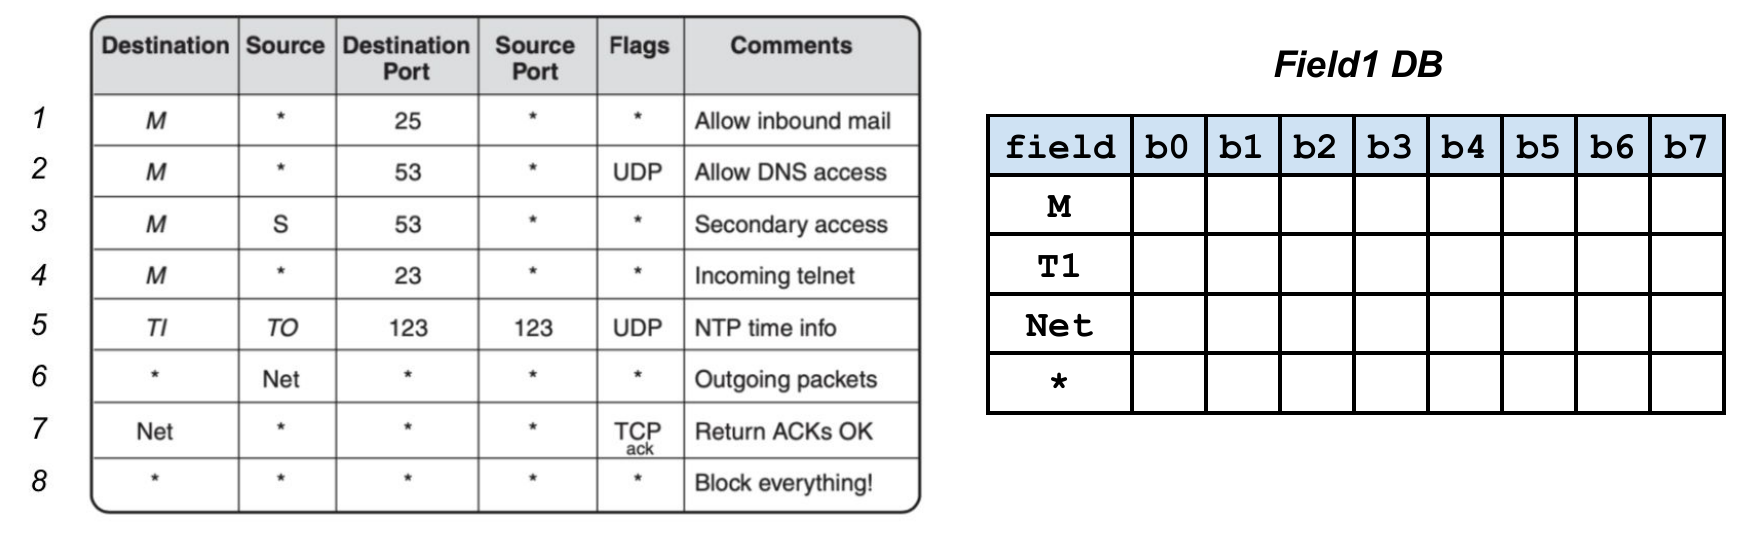
\includegraphics[scale=0.5]{../../immagini/bvls}
\end{figure}\\\\
facciamo questa operazione per ogni DB individuale.
\\Per fare l'intersezione, si mettono in AND tutte le maschere e la regola presa sarà il bit più significativo pari ad 1.
\\Per trovare questo bit più significativo, possiamo costruire una tabella pre-computata ma anche qui la richiesta di memoria creace esponenzialmente.
\\Ma non abbiamo bisogno di salvare tutte le combinazioni, se basta vedere solo il primo bit settato ad 1, basta salvare solo quello: \textbf{Algoritmo di de Bruijn}
\begin{itemize}
\item isoliamo il bit ad 1 più significativo, facendo $x \& (-x)$
\item definiamo una funzione di hash per indicizzare n diverse "parole ad un 1":
    \begin{equation}
        h(z) = z * Debruijn >> (n - 2log_2(n))
    \end{equation}
\item infine, si trova l'indice dell'ordine più piccolo di x: index = $h(x \& (-x))$
\end{itemize}
Le performance dell'algoritmo
\begin{itemize}
\item N regole, le bitmap intersecate sono di N bit, quindi l'AND richiede O(N);
\item calcolare l'AND di K vettori lunghi N bit richiede O(N*K), ma in realtà le CPU a 64 bit fanno un lookup in un ciclo di clock, quindi è $O(N*\frac{K}{W})$, dove W è la larghezza di banda
\item 
\end{itemize}


\paragraph{Rule Cross Product} Creiamo tutte le possibili combinazioni variando tutte le possibili entry di un campo quando c'è una wildcard, ma di nuovo c'è un problema di esplosione della memoria.
\\Ci sono ottimizzazioni, in quanto gli attuali cross products sono tanti, ma in realtà le classi ottenute da queste sono molte meno e quindi possiamo \textbf{Equivalence Cross-Producting}, in quanto se consideriamo il cross product di diversi campi, questi possono portare ad una stessa regola, quindi si identifica una classification class ed il numero di queste è molto minore del totale dei cross products.
\\Quindi si riduce l'occupazione di memoria in maniera significativa, ma quello fatto fin ora è solo sui campi degli IP, occorre unire gli altri e poi fare quello che veniva fatto anche nel linear search bit vector.\\

\paragraph{Decision Tree}
L'idea è di creare un albero di decisione per arrivare alle regole scartandone alcune (??), qualcosa del genere.

\section{Linear Bit Vector Firewall con eBPF/XDP}
Implementare l'algoritmo di ricerca lineare con bit vector usando eBPF.
\\eBPF è un framework originariamente sviluppato per Linux con cui è possibile scrivere dei piccoli programmi di rete in linguaggi di alto livello, si compila il programma e si inietta il bytecode generato all'interno di specifici hooks del kernel.
\\Il programma viene eseguito nel kernel ma in una sandbox, quindi ci sono importanti aspetti di sicurezza.
\\È possibile inoltre interagire col programma, ci sono differenti interfacce, dette \textbf{maps} che possono essere lette e scritte sia dal kernel space che dallo user space.
\subsection{Hooks e programmi}
I programmi eBPF sono guidati ad eventi, l'evento che triggera l'hook è l'arrivo di un pacchetto: questo viene processato dall'hook e poi si passa al prossimo.
\\L'hook più interessante è l'XDP hook, il più efficiente in quanto si bypassa quasi del tutto lo stack kernel e siamo nella parte più di basso livello dove fare qualcosa col pacchetto.
\\Un programma eBPF si scrive in un linguaggio di alto livello come C (restricted), si usa un compilatore come \texttt{llvm} e si compila il programma di ePBF.
\\Si ottiene un bytecode per un'architettura virtuale in grado di processare l'instruction set di eBPF: quando viene iniettato il bytecode nel kernel si ricompila il binario nell'ISA della macchina host col JIT compiler.
\\La syscall \texttt{bpf} inietta il codice nel kernel:
\begin{itemize}
\item la prima cosa che fa il kernel è la verifica del programma, quindi verifica staticamente se non ci sono eccezioni dovute a letture di memoria errate etc... Ci sono varie altre limitazioni; 
\item viene chiamato il JIT;
\end{itemize}
Le due componenti fondamentali di eBPF sono
\begin{itemize}
\item maps: strutture di tipo key:value scrivibili/leggibili sia lato kernel che user. il ruolo delle mappe è almeno duplice
\begin{itemize}
\item salvare dello stato riguardo l'esecuzione;
\item configurare il programma, se ad esempio c'è una routing table si può cambiare a run time
\end{itemize}
\item helper function: ci sono varie funzioni helper, ad esempio per accedere alla mappa. Sono come delle syscall implementate in dei moduli appositi del kernel.
\end{itemize}

\section*{LAB eBPF}
Occorre fare tutti i controlli sugli accessi di memoria, altrimenti al caricamento del modulo nel kernel si ottiene un errore dopo i controlli effettuati dal kernel. XDP può essere usato in parallelo, la stat\_db map è globale quindi è sharata fra le diverse istanze e quindi occorre mettere un lock per garantire la mutua esclusione degli accessi concorrenti.\\ Le limitazioni del lab sono le seguenti
\begin{itemize}
\item il DB è piccolo, solo 32 regole
\item la ricerca è lineare per trovare il bit più significativo
\item l'adattamento delle regole è statico
\end{itemize}
Ci sono delle possibili estensioni (ovviamente, scritte nelle slides)

\end{document}
